\documentclass{beamer}

\mode<presentation>{
\usetheme{CambridgeUS}
}


\usepackage[utf8]{inputenc}
\usepackage[ngerman]{babel}
\usepackage{graphicx}
\usepackage{wrapfig}


\title [] {Musikdownloads \\ Geschichte, Formate, Geschäftsmodelle}
\author [Baumgartner/Krall] {Martin Baumgartner, Daniel Krall}
\institute[Universität Salzburg]{Universität Salzburg}
\date{\today}
%--------------------------------------------------------------------------------
%--------------------------------------------------------------------------------
%--------------------------------------------------------------------------------
\begin{document}
%--------------------------------------------------------------------------------

\begin{frame}
\titlepage

\end{frame}

\begin{frame}
\frametitle{Übersicht}
\begin{itemize}
\Large	
\item  Geschichte der Tonaufnahme
\item  Verlustfreie Audio-Formate
\item  Verlustbehaftete Audio-Formate
\item  Geschäftsmodelle
\end{itemize}
\end{frame}
%--------------------------------------------------------------------------------
\section{Geschichte}
%--------------------------------------------------------------------------------

\begin{frame}
\frametitle{Anfang 1800: Erste Entdeckung}

\begin{columns}
	\column{0.5\linewidth}
	\begin{itemize}
	\Large
	\item Jean Marie Constant Duhamel
	\vspace{0.5cm}\item Bleistift\\ \hspace{0.7cm}\textbf{+}\\Stimmgabel\\ \hspace{0.7cm}\textbf{+}\\Vibration\\ \hspace{0.7cm}\textbf{=}\\Wellenlinien
	\end{itemize}
	\column{0.5\linewidth}
	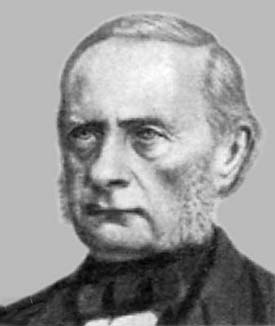
\includegraphics[width = 5cm,height=5cm]{../../Downloads/JMC_Duhamel.jpg}
\end{columns}
\end{frame}
%--------------------------------------------------------------------------------
\begin{frame}
\frametitle{Weiterentwicklung}

\begin{columns}
	\column{0.7\linewidth}
	\begin{itemize}
	\Large
	\item Thomas Young
		\begin{itemize}
		\item 1773-1829
		 \item Augenarzt/Physiker
		\end{itemize}
		
		\vspace{0.5cm}\item Kymograph(Wellenschreiber)
		\begin{itemize}
		\item nicht Abspielbar
		\item Vorläufer Phonograph
		\end{itemize}					
	\end{itemize}
	\column{0.3\linewidth}
		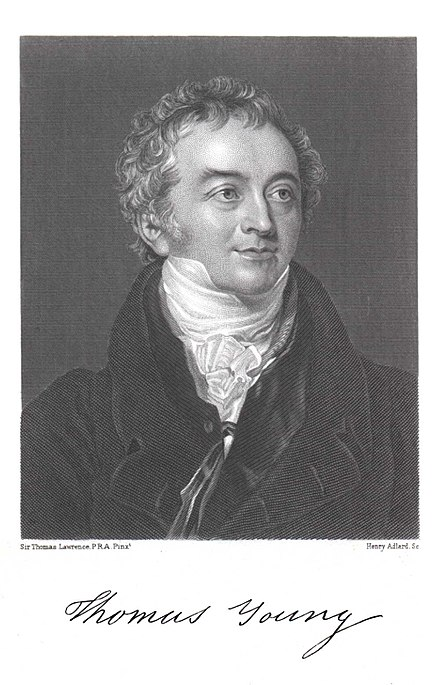
\includegraphics[width=3cm,height=4cm]{../../Downloads/thomas young.jpg} 
		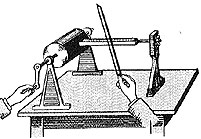
\includegraphics[width=3cm,height=2cm]{../../Downloads/Kymograph_Thomas_Young_1807.png} 
\end{columns}	
\end{frame}
%--------------------------------------------------------------------------------

\begin{frame}
\frametitle{Die älteste erhaltene Tonaufnahme}
\begin{columns}
	\column{0.7\linewidth}
	\begin{itemize}
	\Large	
	\item Édouard-Léon Scott de Martinville
		\begin{itemize}
		\item Drucker
		\item Buchhändler
		\item Erfinder
		\end{itemize}		
	\vspace{0.5cm}\item Phonautograph
	\vspace{0.5cm}\item Au clair de la lune 1860					
	\end{itemize}
	\column{0.3\linewidth}
		\includegraphics[width=3cm,height=3cm]{../../Downloads/Edouard-Léon_Scott_de_Martinville.jpg} 
		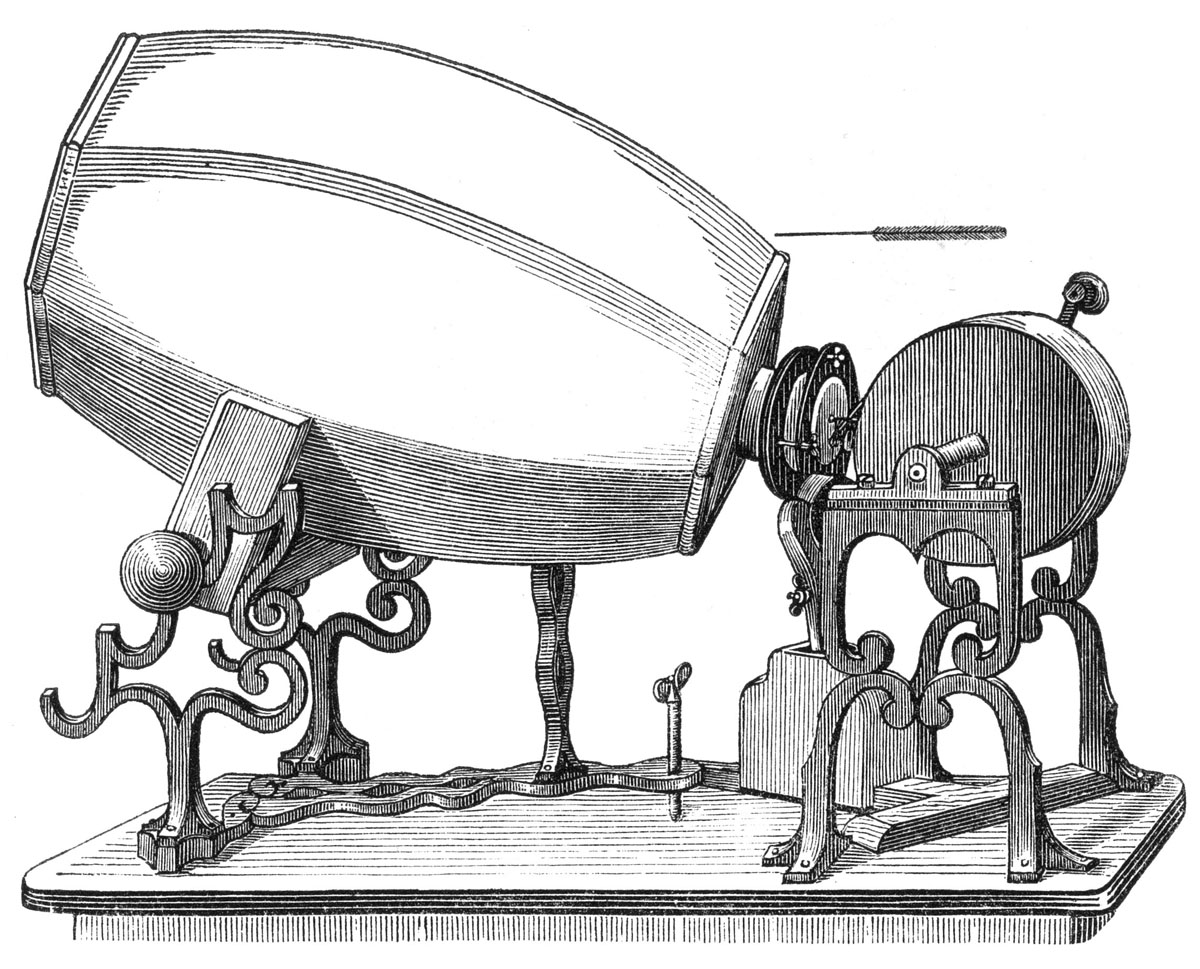
\includegraphics[width=3cm,height=3cm]{../../Downloads/Phonautograph_1859.jpg} 
\end{columns}	

\end{frame}
%--------------------------------------------------------------------------------

\begin{frame}
\frametitle{Das Telegraphon}
\begin{columns}
	\column{0.7\linewidth}
	\begin{itemize}
		\Large		
		\item 1898		
		\vspace{0.5cm}\item Valdemar Poulsen
		\vspace{0.5cm}\item Erstes funktionsfähiges Gerät
		\begin{itemize}
			\item Elektromagnetische Induktion
		\end{itemize}							
	\end{itemize}
	\column{0.3\linewidth}
		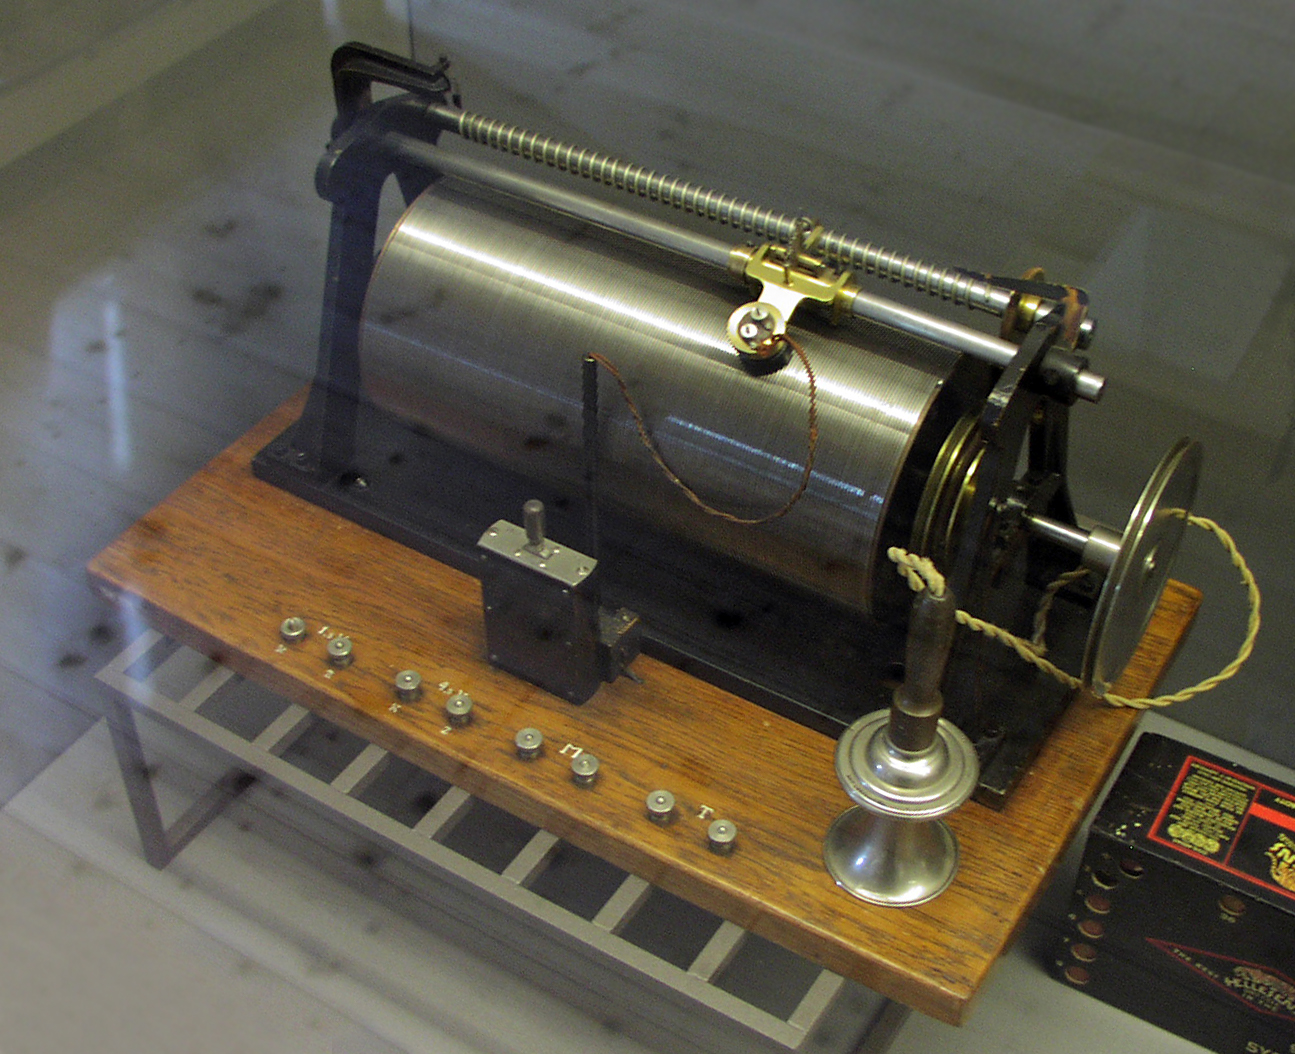
\includegraphics[width=3cm,height=3cm]{../../Downloads/Telegrafon_8154-2.jpg} 
		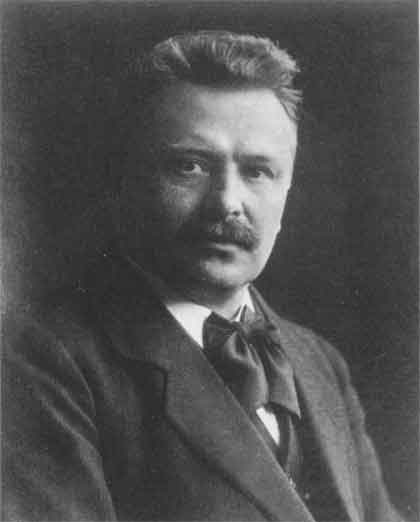
\includegraphics[width=3cm,height=3cm]{../../Downloads/ValdemarPoulsen.jpg} 
\end{columns}	
\end{frame}
%--------------------------------------------------------------------------------

\begin{frame}
\frametitle{Erste Tonbandgeräte}
\begin{columns}
	\column{0.6\linewidth}
	\begin{itemize}
		\Large		
		\item Magnetophon
		\begin{itemize}
			\item 1935
			\item Firma AEG
		\end{itemize}				
		\vspace{0.5cm}\item Bestehend aus:
		\begin{itemize}
			\item dünnem Kunststof
			\item magnetisierbarer Schicht
		\end{itemize}							
	\end{itemize}
	\column{0.4\linewidth}
		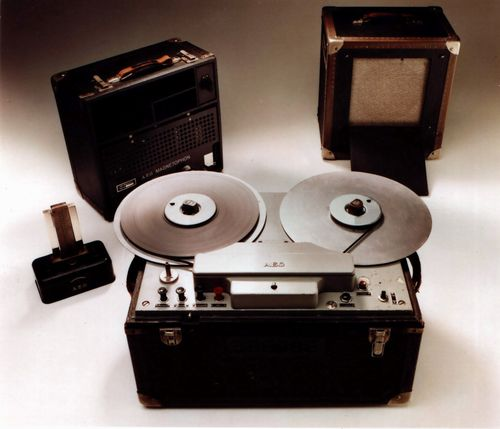
\includegraphics[width=4cm,height=4cm]{../../Downloads/AEG-Magetophon-1935-01.jpg} 
\end{columns}
\end{frame}
%--------------------------------------------------------------------------------

\begin{frame}
\frametitle{Kassettenrekorder}
\begin{columns}
	\column{0.7\linewidth}
	\begin{itemize}
		\Large		
		\item 1963		
		\vspace{0.5cm}\item Tonaufzeichnung:
			\begin{itemize}
				\item analog auf Komaktkassetten
			\end{itemize}
		\vspace{0.5cm}\item Entwickler: Phillips
		\vspace{0.5cm}\item sehr beliebt 1970							
	\end{itemize}
	\column{0.3\linewidth}
		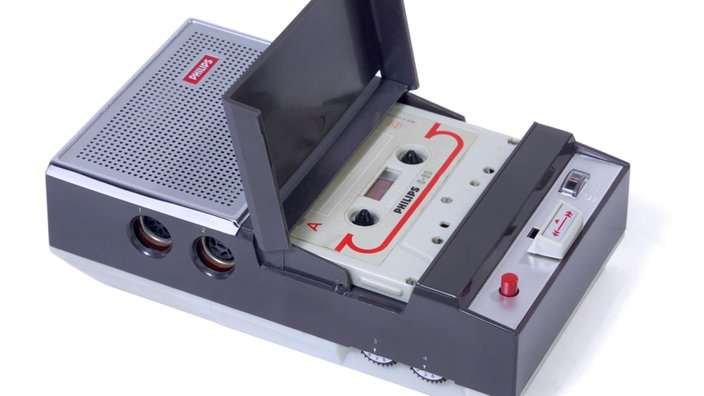
\includegraphics[width=3cm,height=3cm]{../../Downloads/der erste kassettenrekorder.jpg}  
		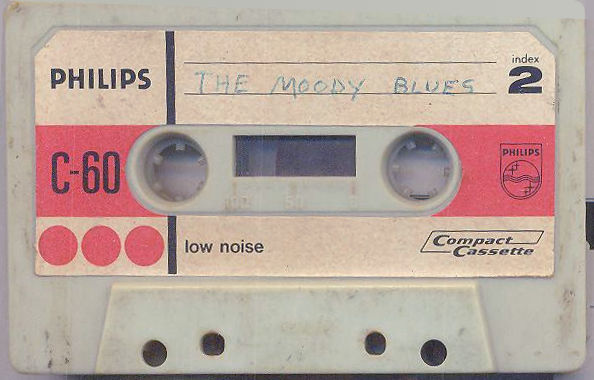
\includegraphics[width=3cm,height=2cm]{../../Downloads/kompaktkassette.jpg} 
\end{columns}	
\end{frame}
%--------------------------------------------------------------------------------

\begin{frame}
\frametitle{Verbreitete körperlose Formate}
\begin{itemize}
	\centering	
	\Large	
	\item .wav
	\vspace{0.5cm}\item .aif
	\vspace{0.5cm}\item .flac
	\vspace{0.5cm}\item ALAC
	\vspace{0.5cm}\item MP3
	\vspace{0.5cm}\item .aac
	\vspace{0.5cm}\item Ogg Vorbis
\end{itemize}
\end{frame}
%--------------------------------------------------------------------------------
\section{Formate}
\subsection{Verlustfrei}
%--------------------------------------------------------------------------------

\begin{frame}
\frametitle{.wav}
\begin{itemize}
	\Large	
	\item Basierend auf RIFF
	\vspace{0.5cm}\item Entwickler: Microsoft, IBM	
	\vspace{0.5cm}\item Unkomprimierte Audiosignale\\(Pulsecodemodulation(PCM))
	\vspace{0.5cm}\item Aus Datenpaketen zusammengesetzt(Chunks)
	\vspace{0.5cm}\item Große Dateien
\end{itemize}
\end{frame}
%--------------------------------------------------------------------------------

\begin{frame}
\frametitle{.aif}
\begin{itemize}
	\Large
	\item Ähnlich wie .wav
	\vspace{0.5cm}\item Entwickler: Apple
	\vspace{0.5cm}\item ID3-Tags
\end{itemize}

\end{frame}
%--------------------------------------------------------------------------------

\begin{frame}
\frametitle{.flac}
\begin{itemize}
	\Large	
	\item Komprimiert(Linear Predictive Coding(LPC))
	\vspace{0.5cm}\item Entwickler: Xiph.org Foundation
	\vspace{0.5cm}\item Open-Source
	\vspace{0.5cm}\item Flexibel
	\vspace{0.5cm}\item Für hochauflösende Musik
\end{itemize}	
\end{frame}
%--------------------------------------------------------------------------------

\begin{frame}
\frametitle{ALAC}
\begin{itemize}
	\Large
	\item MP4 Container
	\vspace{0.5cm}\item Entwickler: Apple
	\vspace{0.5cm}\item basierend auf LPC
	\vspace{0.5cm}\item in Musikstudios weit verbreitet
\end{itemize}
\end{frame}
%--------------------------------------------------------------------------------
\subsection{Verlustbehaftet}
%--------------------------------------------------------------------------------


\begin{frame}
\frametitle{MP3}
\begin{columns}
	\column{0.5\linewidth}
	\begin{itemize}
		\Large		
		\item entwickelt in Erlangen(DE)
		\vspace{0.5cm}\item auf menschliches Gehör angepasst
		\vspace{0.5cm}\item dominierendes Verfahren
		\vspace{0.5cm}\item Standard-MP3: 2 Kanäle
		\vspace{0.5cm}\item seit 2017 frei verfügbar										
	\end{itemize}
	\column{0.5\linewidth}
	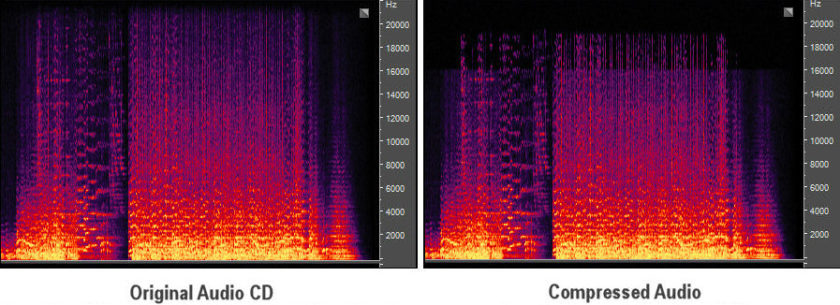
\includegraphics[width=5cm,height=3cm]{../../Downloads/Lossy-vs-Lossless-Spectrum-Analysis-840x305.jpg}  
		 
\end{columns}	
\end{frame}
%--------------------------------------------------------------------------------

\begin{frame}
\frametitle{.aac}
\begin{itemize}
	\Large	
	\item bessere Qualität als MP3
	\vspace{0.5cm}\item kleinere Datengröße als MP3
	\vspace{0.5cm}\item Entwickler: MPEG
	\vspace{0.5cm}\item Mehrkanalfähig
	\vspace{0.5cm}\item Lizenzpflichtig
\end{itemize}	
\end{frame}
%--------------------------------------------------------------------------------

\begin{frame}
\frametitle{Ogg Vorbis}
\begin{itemize}
	\Large	
	\item Patentfrei
	\vspace{0.5cm}\item Entwickler: Xiph.org Foundation
	\vspace{0.5cm}\item ähnlich zu MP3 und AAC
	\vspace{0.5cm}\item Verwendung:
	\begin{itemize}
		\item Spotify
		\item Wikipedia
		\item Internetradio
	\end{itemize}
\end{itemize}	
\end{frame}
%--------------------------------------------------------------------------------
\section{Geschäftsmodelle}
%--------------------------------------------------------------------------------


\begin{frame}
\frametitle{DRM-System}
\begin{columns}
\column{0.5\linewidth}
	\begin{itemize}
		\Large	
		\item Digital Right Management System
		\vspace{0.5cm}\item gegen unbeschränktes weiterverbreiten digitaler Medien
		\vspace{0.5cm}\item digitaler Schlüssel wird verwendet
	\end{itemize}
\column{0.5\linewidth}	
	\includegraphics[width=5.5cm,height=4cm]{../../Downloads/DRMS.png} 
\end{columns}
\end{frame}
%--------------------------------------------------------------------------------

\begin{frame}
\frametitle{À la carte}
\begin{columns}
\column{0.5\linewidth}
	\begin{itemize}
		\Large	
		\item bezahlen dann downloaden
		\vspace{0.5cm}\item meist gratis Hörprobe
		\vspace{0.5cm}\item mit oder ohne DRM
	\end{itemize}
\column{0.5\linewidth}	
	
\includegraphics[width=5.5cm,height=4cm]{../../Downloads/musik-runterladen.jpg}
	\begin{flushright}
		\footnotesize Bild Quelle: Preisgenau.de 
	\end{flushright}	 
\end{columns}	
\end{frame}
%--------------------------------------------------------------------------------

\begin{frame}
\frametitle{Abonnement}
\begin{itemize}
	\Large	
	\item Fixbeitrag
	\vspace{0.5cm}\item Festgelegte Anzahl der zu Downloadenden Inhalte
	\vspace{0.5cm}\item eher Hörbücher
\end{itemize}	
\end{frame}
%--------------------------------------------------------------------------------

\begin{frame}
\frametitle{Flatrate}
\begin{itemize}
	\Large	
	\item monatlicher Beitrag
	\vspace{0.5cm}\item Download unbegrenzt
	\vspace{0.5cm}\item Meist DRM geschützt
\end{itemize}	
\end{frame}
%--------------------------------------------------------------------------------

\begin{frame}
\frametitle{Streaming}
\begin{itemize}
	\Large	
	\item monatliche Gebühr oder kostenlos(mit Werbung)
	\vspace{0.5cm}\item beliebig viele Titel und Alben
	\vspace{0.5cm}\item Playlists nach Belieben
	\item oft mit Flatrate kombiniert
\end{itemize}	
\end{frame}
%--------------------------------------------------------------------------------
\section{Abspann}
%--------------------------------------------------------------------------------

\begin{frame}
\frametitle{Schlussgedanken}
\begin{itemize}
	\Large	
	\item ein sich immer schneller entwickelndes Gebiet
	\vspace{0.5cm}\item kein universelles Format
	\vspace{0.5cm}\item hoher Wettbewerb in der Branche
\end{itemize}	
\end{frame}
%--------------------------------------------------------------------------------

\begin{frame}
\frametitle{ENDE}
\centering 
\Huge
Vielen Dank\\
\vspace{3cm}
\normalsize unmarkierte Bilder, Quelle: Wikipedia
\end{frame}
%--------------------------------------------------------------------------------
\end{document}

